% This file was created by matlab2tikz.
%
%The latest updates can be retrieved from
%  http://www.mathworks.com/matlabcentral/fileexchange/22022-matlab2tikz-matlab2tikz
%where you can also make suggestions and rate matlab2tikz.
%
\definecolor{mycolor1}{rgb}{0.00000,0.44700,0.74100}%
\definecolor{mycolor2}{rgb}{0.85000,0.32500,0.09800}%
\definecolor{mycolor3}{rgb}{0.92900,0.69400,0.12500}%
\definecolor{mycolor4}{rgb}{0.49400,0.18400,0.55600}%
\definecolor{mycolor5}{rgb}{0.46600,0.67400,0.18800}%
%
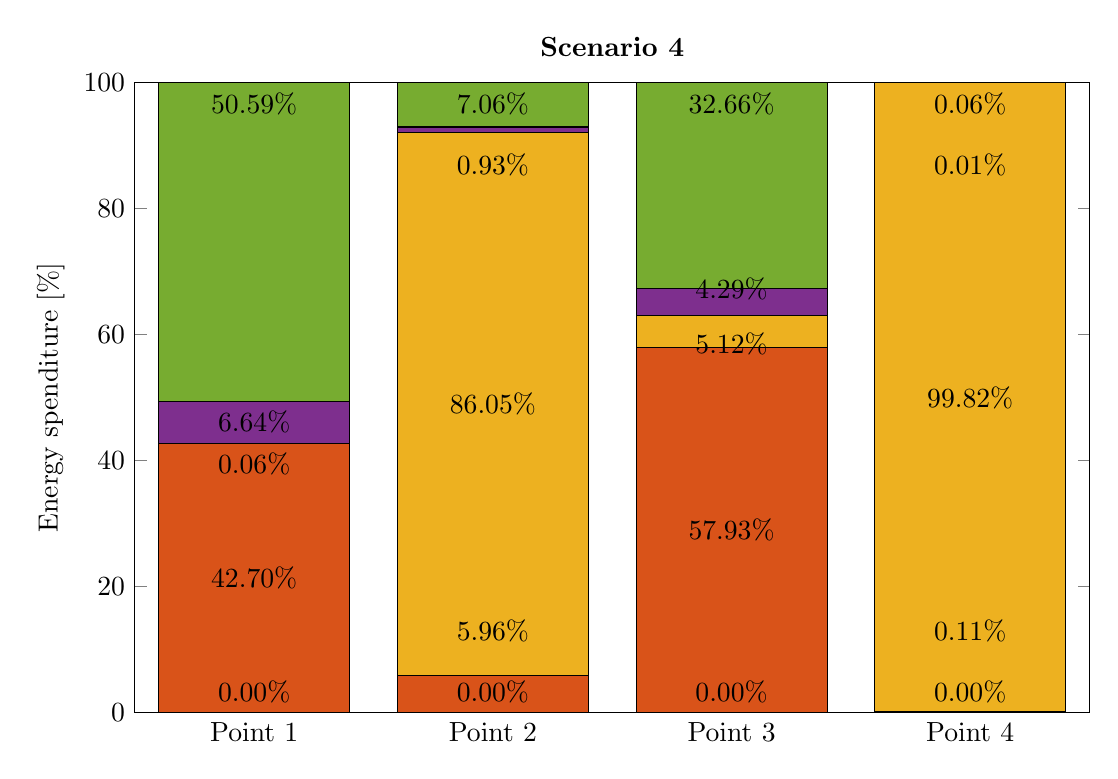
\begin{tikzpicture}

\begin{axis}[%
width=\textwidth,
height=0.66\textwidth,
at={(0.758in,0.481in)},
scale only axis,
bar width=0.8,
xmin=0.5,
xmax=4.5,
xtick={1,2,3,4},
xticklabels={Point 1,Point 2,Point 3,Point 4},
ymin=0,
ymax=100,
ylabel={Energy spenditure [\%]},
axis background/.style={fill=white},
title style={font=\bfseries},
title={Scenario 4}
]
\addplot[ybar stacked,draw=black,fill=mycolor1,area legend] plot table[row sep=crcr] {%
1	0.0002213549734827\\
2	3.09105458526233e-05\\
3	0.000142873785362242\\
4	2.7828337143635e-07\\
};
\addplot[ybar stacked,draw=black,fill=mycolor2,area legend] plot table[row sep=crcr] {%
1	42.700480398537\\
2	5.96279874141242\\
3	57.931115927631\\
4	0.112835718676714\\
};
\addplot[ybar stacked,draw=black,fill=mycolor3,area legend] plot table[row sep=crcr] {%
1	0.0616232156607875\\
2	86.0521542976644\\
3	5.12462755016133\\
4	99.8152760073356\\
};
\addplot[ybar stacked,draw=black,fill=mycolor4,area legend] plot table[row sep=crcr] {%
1	6.64287274338821\\
2	0.927626875949508\\
3	4.28764874624202\\
4	0.0083512965350073\\
};
\addplot[ybar stacked,draw=black,fill=mycolor5,area legend] plot table[row sep=crcr] ;
\node[align=center, text=black]
at (axis cs:1,21.35) {42.70\%};
\node[below, align=center, text=black]
at (axis cs:1,42.732) {0.06\%};
\node[align=center, text=black]
at (axis cs:1,46.084) {6.64\%};
\node[below, align=center, text=black]
at (axis cs:1,100) {50.59\%};
\node[above, align=center, text=black]
at (axis cs:2,0) {0.00\%};
\node[align=center, text=black]
at (axis cs:2,13) {5.96\%};
\node[align=center, text=black]
at (axis cs:2,48.989) {86.05\%};
\node[align=center, text=black]
at (axis cs:2,87) {0.93\%};
\node[below, align=center, text=black]
at (axis cs:2,100) {7.06\%};
\node[above, align=center, text=black]
at (axis cs:3,0) {0.00\%};
\node[align=center, text=black]
at (axis cs:3,28.966) {57.93\%};
\node[align=center, text=black]
at (axis cs:3,58.494) {5.12\%};
\node[align=center, text=black]
at (axis cs:3,67.2) {4.29\%};
\node[below, align=center, text=black]
at (axis cs:3,100) {32.66\%};
\node[above, align=center, text=black]
at (axis cs:4,0) {0.00\%};
\node[align=center, text=black]
at (axis cs:4,13) {0.11\%};
\node[align=center, text=black]
at (axis cs:4,50.02) {99.82\%};
\node[align=center, text=black]
at (axis cs:4,87) {0.01\%};
\node[below, align=center, text=black]
at (axis cs:4,100) {0.06\%};
\end{axis}
\end{tikzpicture}%